\section{Tipos de Dados e Instruções Primitivas}


\begin{frame}{Resumo}
    \fontsize{12pt}{15}\selectfont{
    A partir deste ponto de estudo, teremos contato direto com a parte mais prática desta disciplina. Anteriormente, apresentou-se uma teoria básica de alguns pontos que, por vezes, levaram dúvidas até a alguns profissionais experientes da área de tecnologia da informação.
        
	}\par
	\vspace{1em}
\end{frame}



\begin{frame}{Tipos de informação}
    \fontsize{12pt}{15}\selectfont{
    Daqui pra frente é necessário considerar que um computador é uma ferramenta para solucionar problemas que envolvam a manipulação de informação, as quais se classificam, grosso modo, em dois tipos básicos: dados e instruções.
        
	}\par
	\vspace{1em}
\end{frame}


\begin{frame}{Tipos de dados}
    \fontsize{13pt}{15}\selectfont{
    Os dados são representados por elementos advindos do mundo externo, os quais representam as informações que os seres humanos manipulam. Eles devem ser abstraídos para serem processados em um computador. Os dados podem ser categorizados em três tipos: numéricos, caracteres e lógicos.
        
	}\par
	\vspace{1em}
\end{frame}


\begin{frame}{Tipos de dados}
    \fontsize{13pt}{15}\selectfont{
        \begin{itemize}
            \item \textbf{Numéricos} - representados por valores inteiros ou reais.
            \item \textbf{Caracteres} - representados por valores alfabéticos ou alfanuméricos os quais não são utilizados em operações de cálculo matemático.
            \item \textbf{Lógicos} - representados por valores dos tipos falsos ou verdadeiro.
        \end{itemize}
        
	}\par
	\vspace{1em}
	*Os tipos de dados \textbf{numérico inteiro}, \textbf{numérico real}, \textbf{caracteres} e \textbf{lógico} são conhecidos como tipos de \textbf{dados primitivos} ou tipos de \textbf{dados básicos}.
	\vspace{1em}
\end{frame}

\begin{frame}{Tipos de dados NUMÉRICOS}
    \fontsize{13pt}{15}\selectfont{
        São tipos de dados numéricos possuem duas classes, números inteiros e reais.
	}\par
	\fontsize{12pt}{15}\selectfont{
	    \begin{itemize}
	        \item \textbf{INTEIRO} - são inteiros os dados numéricos positivos e negativos pertencentes ao \textbf{conjunto de números inteiros}, excluindo qualquer valor numérico fracionário, como por exemplo: R\$ 3,19 (não inteiro, fracionário).
	        
	        \item \textbf{REAL} - são reais os dados numéricos positivos e negativos pertencentes ao \textbf{conjunto de números reais}, incluindo todos os valores fracionários e também os valores inteiros, como por exemplo: R\$ 3,19 (não inteiro, fracionário, real).
	    \end{itemize}
	}\par
	\vspace{1em}
\end{frame}


\begin{frame}{Tipo de dados - CARACTERES}
    \fontsize{12pt}{15}\selectfont{
        Os tipos de caracteres são sequência de valores delimitados por aspas formadas por letras de (A até Z), números (|de 0 até 9|) e símbolos - todos os símbolos do teclado. Ele também é conhecido como \textbf{alfanumérico}, \textbf{string} (em inglês - cordão, colar), \textbf{literal} ou \textbf{cadeia}.
        
        Por exemplo, ``Rua João e Maria''.
        
	}\par
	\vspace{1em}
\end{frame}


\begin{frame}{Tipo de dados - LÓGICOS}
    \fontsize{12pt}{15}\selectfont{
        São lógicos os dados com valores que sugerem uma única opção entre duas possibilidades existentes, normalmente representados pelos valores \textbf{FALSO} ou \textbf{VERDADEIRO}, podendo também ser representados por \textbf{SIM} ou \textbf{NÃO}, \textbf{1 (um)} ou \textbf{0 (zero)}, entre outros, desde que mantida a relação de escolher apenas uma das duas opções de possibilidade existentes. 
        
        Ele também é conhecido por \textbf{booleano}, devido à contribuição de George Boole.
	}\par
	\vspace{1em}
\end{frame}


\begin{frame}{O uso de variáveis}
    \fontsize{12pt}{15}\selectfont{
        Tem-se como definição de variável tudo aquilo que é sujeito a variação, que é incerto, instável ou inconstante.
        
        \vspace{1em}
        Para utilizar o conceito de variável, imagine que a memória de um computador é um grande arquivo com várias gavetas, e cada gaveta pode armazenar um único valor (seja ele numérico, caractere ou lógico).
	}\par
	\vspace{1em}
\end{frame}


\begin{frame}{O uso de variáveis}
	\vspace{1em}
	\centering
    
\includegraphics[width=0.7\textwidth]{images/fig-gavetas.jpg}
\end{frame}


\begin{frame}{O uso de variáveis}
    \fontsize{14pt}{15}\selectfont{
        Se a memória do computador for comparado a um grande arquivo com várias gavetas, e em cada gaveta é possível guardar um único valor por vez. Como em um arquivo, as gavetas devem estar identificadas com uma etiqueta contendo um nome. 
        \vspace{1em}
        
        Você há de concordar que é necessário identificar com um nome a gaveta que se pretende utilizar. Desta forma o valor armazenado pode ser utilizado a qualquer momento.
        
	}\par
	\vspace{1em}
\end{frame}


\begin{frame}{O uso de variáveis}
	\vspace{1em}
	\centering
    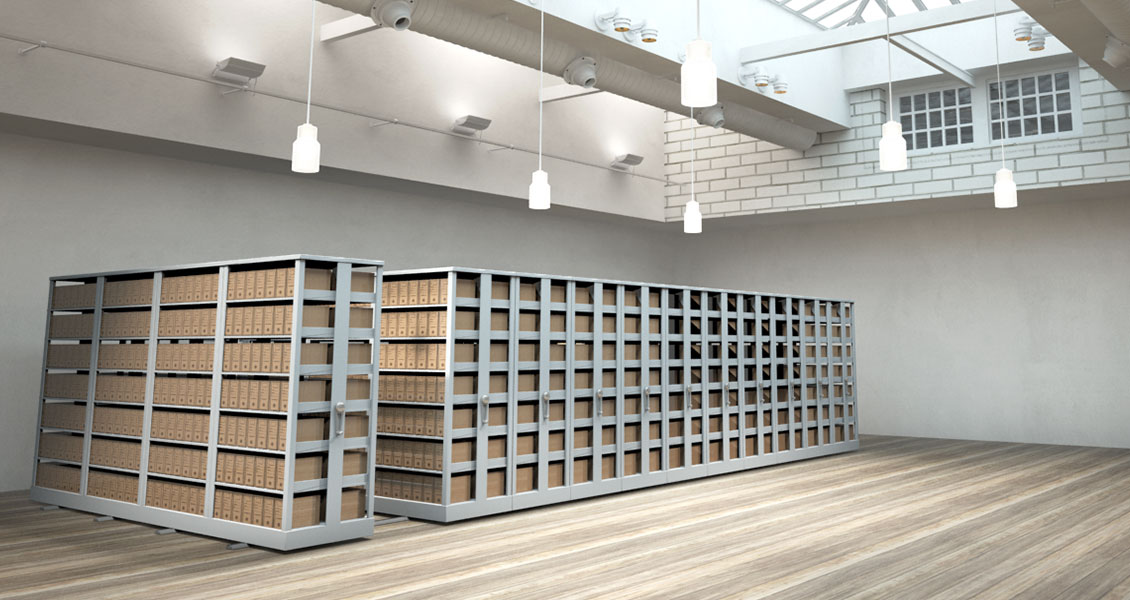
\includegraphics[width=0.8\textwidth]{images/fig-arquivo-gavetas.jpg}
\end{frame}




\begin{frame}{O uso de variáveis}
    \fontsize{14pt}{15}\selectfont{
        O nome de uma variável é utilizado para sua identificação e representação dentro de um programa de computador. É necessário estabelecer e seguir algumas regras de definição e uso de variáveis, a saber:
        
        \vspace{1em}
	}\par
	\fontsize{12pt}{15}\selectfont{
	    \begin{itemize}
	        \item Os nomes de identificação de uma variável podem utilizar um ou mais caracteres, limitando-se a restrição da própria linguagem formal de programação em uso. No caso do diagrama de blocos essa restrição não existe.
	    \end{itemize}
	}
	\vspace{1em}
\end{frame}


\begin{frame}{O uso de variáveis}
    \fontsize{14pt}{15}\selectfont{
        (continuação)
        \vspace{1em}
	}\par
	\fontsize{12pt}{15}\selectfont{
	    \begin{itemize}
	        \item O primeiro caractere de identificação do nome de uma variável não pode ser, em hipótese alguma, numérico. O primeiro caractere de identificação do nome de uma variável deve sempre ser alfabético, os demais podem ser alfanuméricos.
	        
	        \item Na definição de um nome composto de uma variável não podem existir espaços em branco entre os nomes. 
	        
	        \item Jamais uma variável pode ser definida com o mesmo nome de uma palavra que representa os comandos de uma linguagem de programação de computador, ou seja, com as palavras reservadas de uma linguagem.
	        
	    \end{itemize}
	}
	\vspace{1em}
\end{frame}



\begin{frame}{O uso de variáveis}
    \fontsize{14pt}{15}\selectfont{
        Por fim, do ponto de vista computacional pode-se definir uma variável de forma bem simplista como uma representação de uma região de memória utilizada para armazenar um determinado valor por um espaço de tempo. O tempo de armazenamento de um valor está relacionado ao tempo de duração da execução de um programa.
        \vspace{1em}
	}\par
	\vspace{1em}
\end{frame}


\begin{frame}{O uso de constantes}
    \fontsize{14pt}{15}\selectfont{
        \textbf{Constante} é tudo que é fixo, estável, inalterável, imutável, contínuo, invariável, de um valor fixo e que é aplicado sob diversos pontos de vista. Assim sendo, do ponto de vista computacional, que é semelhante ao matemático ou científico, uma constante é uma grandeza numérica que mantém-se inalterado.
        \vspace{1em}
	}\par
	\vspace{1em}
\end{frame}



\begin{frame}{Os operadores aritméticos}
    \fontsize{12pt}{15}\selectfont{
        Os operadores aritméticos são as ferramentas responsáveis pelo estabelecimento das operações matemáticas a serem realizadas em um computador. Tanto variáveis como constantes são utilizadas na elaboração dos cálculos matemáticos. Eles são classificados em:
        \vspace{1em}
	}\par
	\fontsize{12pt}{15}\selectfont{
	    \begin{itemize}
	        \item \textbf{unários} - quando atuam na inversão do estado de um valor numérico, que pode este ser passado de positivo para negativo ou de negativo para positivo; ou
	        
	        \item \textbf{binários} - quando utilizados em operações matemáticas de exponenciação, divisão, multiplicação, adição e substração.
	        
	    \end{itemize}
	}
	\vspace{1em}
\end{frame}




\begin{frame}{Os operadores aritméticos}

\resizebox{\linewidth}{!}{
\begin{tabular}{|c|c|c|c|c|}
\hline
\textbf{Operador} & \textbf{Operação}& \textbf{Categoria} & \textbf{Prioridade} & \textbf{Resultado} \\ \hline
=  & Atribuição & -o- & -o-  & -o- \\ \hline
+  & Manutenção de sinal & unário & 1 & -o- \\ \hline
-  & Inversão de sinal& unário & 1 & -o- \\ \hline
\textasciicircum{}& Exponenciação & binário& 2 & inteiro ou real \\ \hline
% \textasciicircum{}(1/n) & Radiciação de índice n & binário& 2 & real\\ \hline
/  & Divisão & binário& 3 & real \\ \hline
*  & Multiplicação & binário& 3 & inteiro ou real \\ \hline
+  & Adição  & binário& 4 & inteiro ou real \\ \hline
-  & Subtração  & binário& 4 & inteiro ou real \\ \hline
\end{tabular}
}

*o quadro apresenta os operadores aritméticos segundo a ordem de prioridade matemática em que as operações aritméticas são realizadas. Para alterar o nível de prioridade deve utilizar-se parênteses. Por exemplo, X = 10 * 10 + 2 e Y = 10 * (10 + 2), X tem resultado 102 e Y tem resultado 120.

\end{frame}


\begin{frame}{Instruções Básicas}
    \fontsize{12pt}{15}\selectfont{
        As instruções a serem implementadas para execução de um determinado programa são representadas por um conjunto de palavras-chave (vocabulário). Uma instrução pode se:
        \vspace{1em}
	}\par
	\fontsize{12pt}{15}\selectfont{
	    \begin{itemize}
	        \item \textbf{formal} - quando baseia-se em linguagem real de programação de computadores, tais como C, Java, PHP; ou
	        
	        \item \textbf{informal} - quando baseia-se em pseudocódigo, como é o caso da linguagem usada até, diagrama de blocos.
	        
	    \end{itemize}
	}
	\vspace{1em}
\end{frame}



\begin{frame}{Entrada, Processamento e saída}
    \fontsize{12pt}{15}\selectfont{
        Para criar um programa que seja executável dentro de um computador, é preciso ter em mente três pontos de trabalho:
        \vspace{1em}
	}\par
	\fontsize{12pt}{15}\selectfont{
	    \begin{itemize}
	        \item entrada de dados - alimenta o programa;
	        
	        \item processamento - processa a(s) entrada(s); e
	        
	        \item saída de dados - apresenta o resultado.
	        
	    \end{itemize}
	}
	\vspace{1em}
\end{frame}

